%%%%%%%%%%%%%%%%%%%%%%%%%%%%%%%%%%%%%%%%%%%%%%%%%%%%%%%%%%%%%%%%%%%%%%%%%%%%%%%%%%%%%%%%%%%%%%%%%%%
%
% Notes on Citations
%
% MooreAfter2017.bib is an export of the MooreAfter2017 saved search in my Zotero database.
%
% Make sure that the citekey is pinned to each item ( Right click; Better Bibtex | Pin Bibtex key)
%
% After uploading, click on Tools | Bibliography, then open the log file to see any warnings
% or errors which need to be fixed. 
%
% Fix any problems in Zotero, then export a fresh version of MooreAfter2017.bib
%
%%%%%%%%%%%%%%%%%%%%%%%%%%%%%%%%%%%%%%%%%%%%%%%%%%%%%%%%%%%%%%%%%%%%%%%%%%%%%%%%%%%%%%%%%%%%%%%%%%%
%
% Checking links in PDF
%
% pdfx -c CFES2019.pdf
%
%%%%%%%%%%%%%%%%%%%%%%%%%%%%%%%%%%%%%%%%%%%%%%%%%%%%%%%%%%%%%%%%%%%%%%%%%%%%%%%%%%%%%%%%%%%%%%%%%%%

\documentclass[12pt,english]{scrartcl}
\usepackage[T1]{fontenc}
\usepackage{color}
\usepackage{array}
\usepackage{url}
\usepackage{pdfpages}

\usepackage[utf8]{inputenc}
\usepackage[english]{babel}
\usepackage{csquotes}

% Use style=draft to print citation keys
%\usepackage[defernumbers=true,backend=biber,style=draft]{biblatex}
\usepackage[defernumbers=true,backend=biber]{biblatex}

\addbibresource{MooreAfter2017.bib}
\addbibresource{inat.bib}
\addbibresource{misc.bib}
\usepackage[breaklinks=true, colorlinks=True, allcolors=blue]{hyperref}

\usepackage{indentfirst} 
\usepackage{comment}

% A couple of very simple macros to add 'Activities' and 'Plans' headings.
\newcommand{\activities}{\medskip\textbf{Activities}}
\newcommand{\plans}{\medskip\textbf{Plans}}

\makeatletter

\makeatother

\errorcontextlines=3 % For checking biblatex

\begin{document}

\title{CFES Report 2019}

\author{Aubrey Moore, Ph.D.\\
Professor / Extension Entomologist}

\maketitle

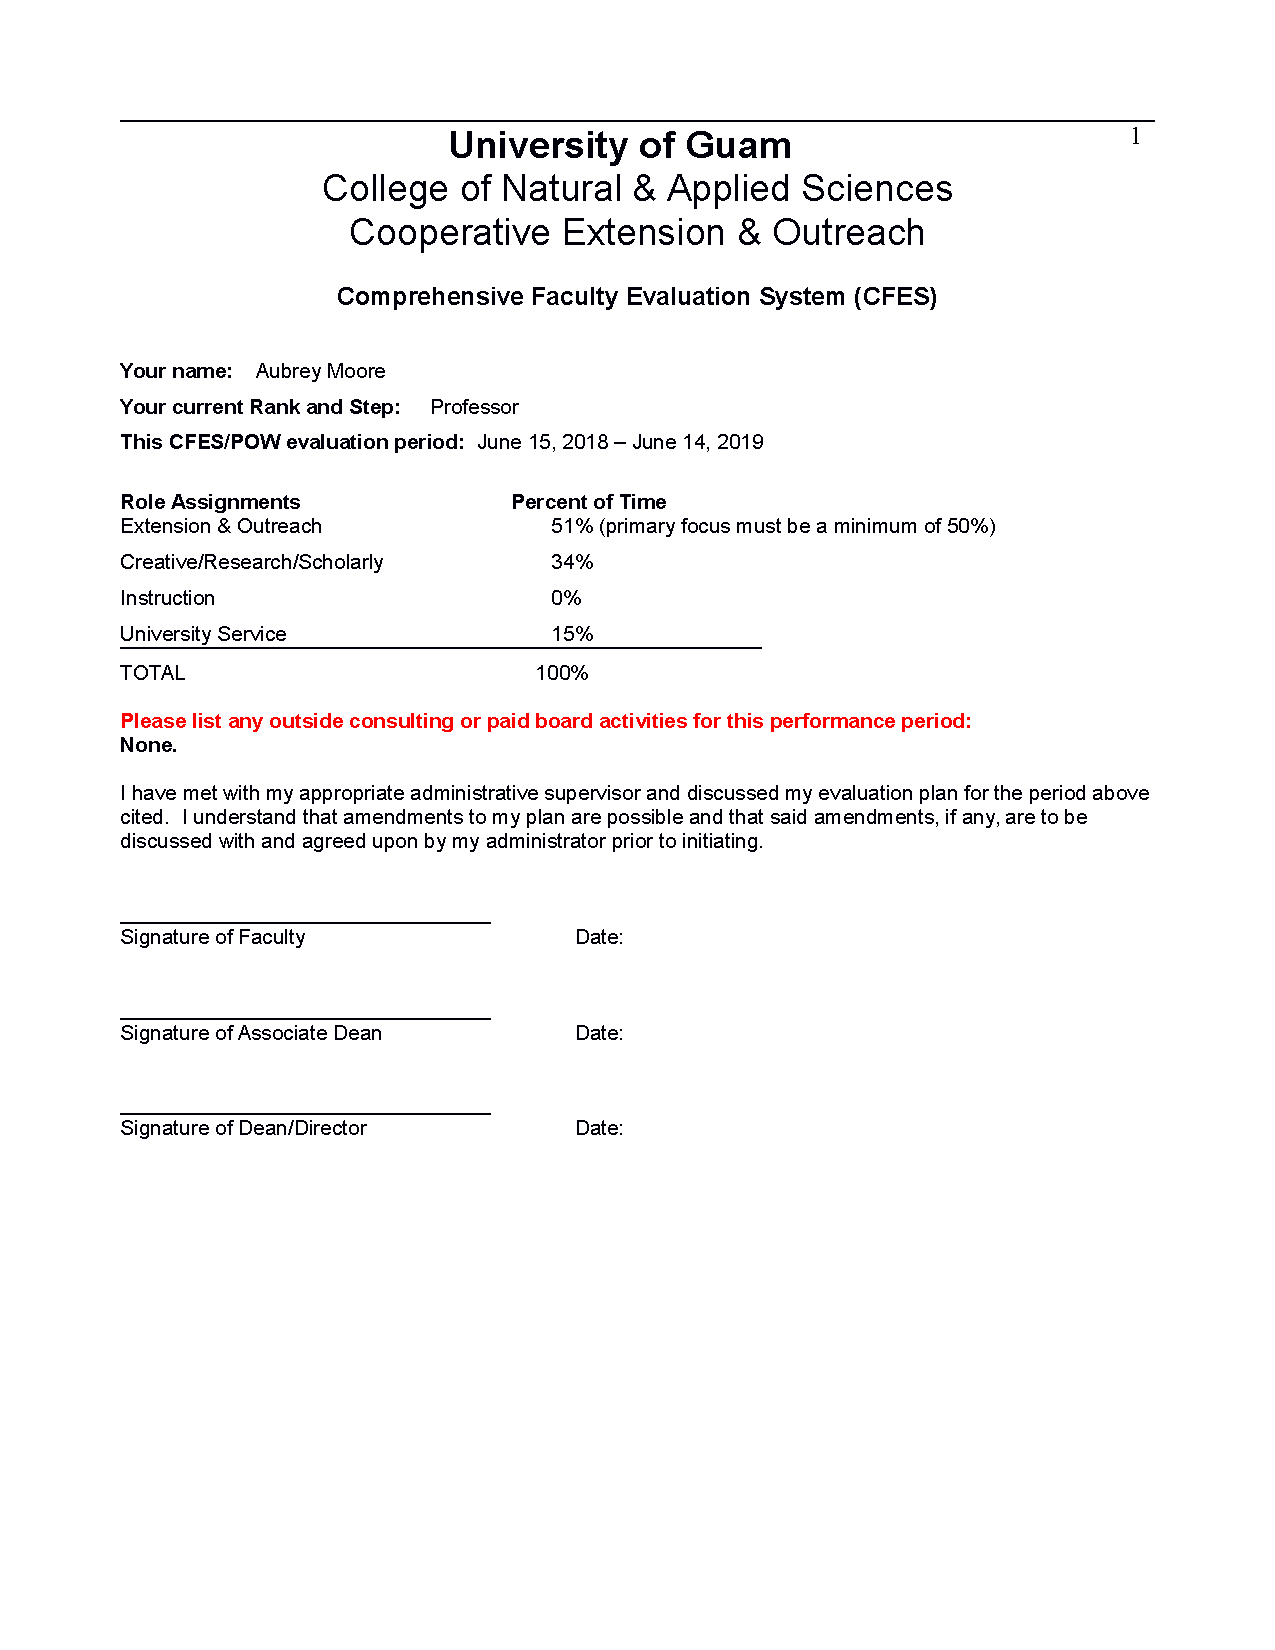
\includepdf[pages=1]{Reflective2019-form}

\tableofcontents{}

\clearpage

\section{Preface}
\begin{refsection}
	
I was hired by the University of Guam on October 1, 2003 under a limited-term,
split appointment (50\% extension and 50\% research). On June 26,
2008, I started a tenure-track appointment as extension entomologist
(100\% extension) with the academic rank of assistant professor. At
the end of the 2012 fall term I applied for tenure and promotion to associate professor and
received both in 2013. At the end of 2018 fall term I applied for promotion to
full professor and was promoted on July 11, 2019~\cite{recommendation_for_promotion2019}. 

I work within the Agriculture and Natural Resources Unit of the University
of Guam Cooperative Extension Service. I am a faculty member of the
Environmental Science Graduate Program and a member of the Western
Pacific Tropical Research Center. 

This report documents my activities from June 15, 2018 through the present.

My current faculty role allocation is as follows:
\begin{itemize}
	\item 51\% Extension and Community Activities 
	\item 34\% Creative/Scholarly Activity or Research 
	\item 15\% University and Community Service
\end{itemize}

\textbf{Note to Reader:}

This report is available as an electronic document in PDF format at\\
\url{https://github.com/aubreymoore/CFES2019/blob/master/CFES2019.pdf}. 

If you are reading the PDF version of the report on a device connected
to the internet, you will be able to follow hypertext links to documents
I have referenced.

\printbibliography

\end{refsection} 

\pagebreak

\section{Extension and Community Activities}

\subsection{Insect Diagnostic Services}
\begin{refsection}
	
As an extension entomologist, a major part of my job is providing
insect identification and pest control recommendations to a diverse
clientele including commercial growers, gardeners, householders, GovGuam
agencies, federal agencies, and UOG colleagues. Most client contacts
are initiated by a phone call or a visit by the client to the ANR
office. In many cases identification and pest control recommendations
require a site visit by me and/or extension associates to collect
samples and define the problem.

\activities

\begin{itemize}
\item The number of extension calls requiring my assistance averaged approximately
three per day during the reporting period. Many of these are documented
as postings to iNaturalist \cite{moore_aubrey_2020}.
\end{itemize}

\plans

\begin{itemize}
\item I plan to continue providing insect diagnostic services.
\end{itemize}

\printbibliography

\end{refsection}


\subsection{Detection and Documentation of Invasive Species}
\begin{refsection}

Invasive insects are arriving on Guam at a very high rate (estimates
range as high as one new species per day). Very few of these are detected
and even fewer are identified because Guam suffers from \href{https://en.wikipedia.org/wiki/Taxonomic_impediment}{the taxonomic impediment}.
Even when reliable species determinations are made, new island records
are only rarely documented in the scientific press. Thus, impacts
of invasive insects on Guam and elsewhere in Micronesia are grossly
underestimated. One of my professional goals is to work towards solving
this problem by increasing the detection rate, getting specimens identified
by qualified taxonomists, and publishing new island records in the
scientific literature.

\activities

\begin{itemize}
	
\item Ten new island records for insects in Micronesia were documented in iNaturalist posts during the reporting period \cite{inat36470788,inat36285968,inat35845152,inat32572967,inat31326484,inat29333274,inat18166461,inat16734728,inat15747194,inat15067449,inat13466275}.

\item New Larval Host Record: \textit{Traminda aventiaria} (Lepidoptera: Geometridae) Feeds on the Critically Endangered Tree, \textit{Serianthes nelsonii} (Leguminosae), on Guam~\cite{moore_new_2020}

\end{itemize}

\plans

\begin{itemize}

\item The International Union for Conservation of Nature (IUCN-ISSG) is
building a Global Register of Introduced and Invasive Species. I have
volunteered to coordinate building a check list for species on Guam.

\item The Guam Invasive Species Council is required to maintain a list on
invasive species on Guam. I have volunteered to be ``registrar''
for this list.

\end{itemize}

\printbibliography
\end{refsection}

\subsection{University of Guam Insect Collection}
\begin{refsection}

The UOG insect collection is a valuable reference collection for extension
entomology, teaching and research. I am a member of the board of directors
for the collection and I work with Dr. Ross Miller to curate and catalog
this collection.

\activities

\begin{itemize}

\item I ported the digital catalog for the UOG Insect Collection from a
CSIRO BioLink database to a more modern web-based Symbiota database
which is now online \cite{moore_scan_2018}.

\item I established an internship to train entomology students how to curate
an institutional insect collection \cite{moore_internship_2018}.

\item The Benita Laird-Hopkins collection includes more than 5,000 insect
specimens reared from seeds of forest plants from Saipan and Guam
as part of the Ecology of Bird Loss Project. This collection has been
cataloged and accessioned into the UOG insect collection and a publication
is being prepared \cite{laird-hopkins_[preparation]_2018}.

\item In June 2018, I attended the Second Annual Digital Data in Biodiversity
Research Conference sponsored by iDigBio (Integrated Digital Biocollections)
to attend a workshop entitled Sharing and Mobilization of Massive
Specimen Image Databases from Collections of Tropical Island Biodiversity
as an invited participant. I made a presentation on building a biodiversity
inventory for Guam \cite{moore_building_2018-1} and discussed ongoing
collaboration with Dr. Alex Vandam on writing an NSF proposal to support
digitization of biological collections on American-affiliated islands
\cite{moore_trip_2018}.
\end{itemize}

\plans

\printbibliography[heading=none]

\end{refsection}

\subsection{Guam Coconut Rhinoceros Beetle Project}

This is my largest and most important project. Please see CRB activities in the Creative/Research/Scholarly section~\ref{sec:Coconut-Rhinoceros-Beetle}.

\subsection{National Plant Diagnostic Network (NPDN)}
\begin{refsection}
	
I serve as the UOG Coordinator for the National Plant Diagnostic Network. 

\activities

\begin{itemize}
\item Participated in monthly conference calls.
\item Prepared an annual work plan and budget \cite{moore_university_2018}.
\item Prepared annual report \cite{moore_npdn_2018}.
\item Served on the NPDN IT Strategic Planning Committee.
\item Trained and certified 14 First Detectors as part of my AL/BI 345 General
Entomology course.
\end{itemize}

\plans

attend meeting in AZ
PIDDRS

\printbibliography[heading=none]

\end{refsection}	

\subsection{Guam Invasive Species Advisory Committee (GISAC) and Guam Invasive Species Council (GISC)}
\begin{refsection}
	
I am a founding member and regular participant in GISAC. President Underwood delegated me to represent UOG as a voting member of GISC.

\activities

\begin{itemize}
	
\item I participated in GISAC and GISC meetings.

\item During 2018, I served on a GISC Import Data Harmonization Committee.
This committee generated recommendations \cite{guerrero_guam_2018}
resulting in a bill to amend the Guam Invasive Species Act \cite{guerrero_bill_2018}.

\end{itemize}

\plans

\begin{itemize}
	
\item I plan to continue as an active member of GISAC and GISC.

\item I plan to participate in a review of the Guam Invasive Speices Management Plan.

\end{itemize}

\printbibliography[heading=none]

\end{refsection}

\subsection{Public Outreach}
	
\subsubsection{Presentations}
\begin{refsection}
	
\nocite{*}
\defbibfilter{presentations}{keyword=presentation2018 or keyword=presentation}
\printbibliography[resetnumbers=true, heading=none,filter=presentations]
\end{refsection} 

\subsubsection{Radio and Newspaper}

\begin{refsection}
	\nocite{*}
	\defbibfilter{press}{keyword=press2018 or keyword=press}
	\printbibliography[filter=press, heading=none]
\end{refsection} 

\begin{comment}

\raggedright\vspace{2mm}\textbf{Activity}
\begin{itemize}
\item Presentations \cite{moore2018building2,blas2018protecting,deloso2018parasitoid,moore2018freecell,moore2018coconut,moore2018biological2,moore2018freecell2,marshall2018progress,moore2018attempted,moore2017impactof,moore2018biological,moore2018building,moore2017invasion,moore2017coconut,moore2017usingfree,moore2017accessto,moore2017biological,moore2017thecoconut,moore2017biological2,moore2017biological3}
\item Workshops \cite{berringer2018sixteenth,moore2017bringyour,moore2018cnasworkshop,quitugua20182018coconut}
\item Press \cite{moore2018special,varietyuogseeks,pacific2018scientists,2018viralcontrol,postnewtree,leonguerrero2018interview,2018g2ghuman,2017tracking}
\end{itemize}
\raggedright\vspace{2mm}\textbf{Reference(s)}

\begin{btSect}[vancouver]{zotero}
\btPrintCited
\end{btSect}
\newpage{}
\end{btUnit}

\begin{btUnit}

\end{comment}

\subsubsection{Internet}

Since the 1990s, I have built and maintained web sites to facilitate sharing information about insects in Micronesia.

\activities

I created a wiki site to serve as an index to web resources I have developed (Available at  \url{https://guaminsects.net/aubwiki2020}).

\plans

I will continue to use web sites to facilitate sharing information on Guam's insects.

\begin{comment}

\raggedright\vspace{2mm}\textbf{Activity}
\begin{itemize}
\item On-line output \cite{moore2018onlinecatalog,moore2018textitcitripestis2,moore2018textitcitripestis,moore2018lobatelac2,moore2018scanuniversity,moore2017website,moore2018insectpin,moore2018checklist,moore2018citripestis,moore2018lobatelac,manuel2017pacific,moore2018inaturalist,moore2018interactive,moore2017listof,moore2017guamforestry,moore2017crbgarticlereview,moore2017crbtrap,moore2017techblog,moore2017scaevoladieback,moore2017failedattempt,moore2017publish,moore2017usingscrapy,moore2017tweeking,moore2017install,moore2017setting,moore2017usingthe,moore2017finding,moore2017usingscrapy2,moore2017calculate,moore2017converting,moore2017migrate,moore2018croppestlist}
\end{itemize}
\raggedright\vspace{2mm}\textbf{Reference(s)}

\begin{btSect}[vancouver]{zotero}
\btPrintCited
\end{btSect}
\newpage{}
\end{comment}

\pagebreak

\section{Creative/Scholarly Activities or Research}

\subsection{\label{sec:Coconut-Rhinoceros-Beetle}Coconut Rhinoceros Beetle (CRB) Biocontrol}
\begin{refsection}
	
\subsubsection{Description}

A newly discovered biotype of coconut rhinoceros beetle (CRB-G) is
rapidly killing coconuts and other palms on Guam and on other Pacific
islands. Following a failed eradication attempt on Guam, CRB-G proved
hard to control because it is resistant to \emph{Oryctes rhinoceros}
nudivirus (OrNV), which was previously used as the preferred biological
control agent for control of CRB outbreaks on Pacific Islands and
elsewhere. Previous to the discovery of CRB-G, all OrNV releases on
Pacific Islands resulted in immediate and sustained suppression of
CRB damage to low levels and prevented tree mortality.

Guam is currently experiencing an uncontrolled and unmonitored island-wide
CRB-G outbreak which was triggered by abundant CRB-G breeding sites
in the form of dead and dying vegetation left in the wake of Typhoon
Dolphin which occured in May 2015. of a recent typhoon. Most of these
breeding sites are inaccessable to sanitation efforts, being either
in the jungle or on military land (which covers one third of Guam).
A positive feedback cycle has begun whereby large numbers of adult
beetles are killing large numbers of palms which become breeding sites
which generate even higher numbers of adults. Severe damage to Guam\textquoteright s
palms prompted the Governor of Guam to declared a state of emergency
in July 2017.

The main objective of this project is to stop the uncontrolled outbreak
on Guam. Entomologists working on the CRB-G problem on several Pacific
islands agree that the most feasible tactic to halt tree mortality
and suppress damage to tolerable levels is establishment of biological
control using an isolate of OrNV which is highly effective as a biological
control agent for CRB-G. We are working with collaborators to identify
populations of CRB-G throughout the Asia-Pacific region. We will sample
these populations for biological control agent candidates which will
be evaluated in laboratory bioassays performed at UOG. Promising candidates
will be field released using autodissemmination as per a USDA-APHIS
import and release permit.

Concurrent with establishment of CRB-G biocontrol, success of the
project will be monitored in a quarterly, island-wide tree health
survey and incidence of OrNV infection will be monitored in a subsample
of all field collected CRB-G.

If the Guam CRB-G infestation cannot be controlled, it is expected
that most palms on the island will be killed and CRB-G will continue
to spread to other islands and beyond. If CRB-G invades smaller islands
and atolls where coconut is the tree of life, a human tragedy will
ensue. On larger islands, coconut and oil palm industries will be
severely impacted. Attempts to organize a regional project in response
to CRB-G are underway.

\subsubsection{Activities}

\paragraph{Funding} This is my largest and most important project, requiring a lot of time and effort for project management including preparation of grant proposals and reports. Funding is currently provided by four grants: USDA-APHIS FY17 Farm Bill~\ref{USDA-APHIS-2017}, USDA-Farm FY18 Bill~\ref{USDA-APHIS-2018}, USDA-Plant Protection Act~\ref{USDA-APHIS-2019} and a grant from the Department of Interior, Office of Insular Affairs~\ref{DOI}. Links to progress reports for these grants are in the appendices. 

I submitted a proposal for FY20 USDA-Plant Protection Act Funds~\ref{USDA-APHIS-2020} and a preproposal for SERDP FY21 funding \ref{SERDP}. 

\paragraph{Staffing}

I am assisted by Dr. James Grasela, and insect pathologist funded by my Department of the Interior Office of Insular Affairs grant \ref{DOI}. Roland Quitugua collaborates on the project with separate funding.  During the reporting period my technician and graduate student, Ian Iriarte, left the University. I have recently hired an entomology student, Christian Cayanan, as a technician.

\paragraph{Current focus} is on finding an isolate of \textit{Oryctes} rhinoceros nudivirus which can be used as a biological control agent for CRB-G. Laboratory bioassays have identified one OrNV isolate which is potential candidate and further tests are under way.

I have developed an online database to facilitate record keeping and report generation for CRB rearing and bioassays \cite{moore_coconut_2019-1}. 

Dr. Grasela has worked in coordination with Dr. Hui Jiang to build DNA diagnostics capacity. We can now test for OrNV in individual beetles.

\paragraph{International collaboration} will be essential for finding a way to halt massive ecological and economic damage to Pacific islands invaded by CRB-G. A CRB-G Action Group has been formed to facilitate collaboration and cooperation.

In August 2018, Moore, Grasela, Quitugua and Iriarte participated in the Congress on Invertebrate Pathology and Microbial Control and the 51st Annual Meeting of the Society for Invertebrate Pathology \cite{moore_trip_2018-1,moore_attempted_2018,marshall_progress_2018}.

During May 2019, Moore travelled to Taiwan to collect CRB-G adults \cite{moore_taipei_2019}. Based on previous research, it seems likely that these beetles will contain OrNV which can be used as a biocontrol agent.

During November 2019, Moore and Grasela participated in the XIX International Plant Protection Congress \cite{moore_india_2019,moore_status_2019,marshall_challenge_2019}.

\paragraph{Outreach} In an effort to facilitate technical and scientific information among people working on CRB, we have developed and maintain several online resources including a wiki \cite{moore_crb-g_2019}, a Facebook site \cite{moore_facebook_2019}, an online interactive map of CRB invasion history \cite{moore_online_2019} and a CRB bibliography \cite{moore_coconut_2019}.

\subsubsection{Plans}

Plans for this project are contingent on applied research results, availability of funding and availability of resources.

\paragraph{Funding} I have submitted a proposal for FY20 USDA-Plant Protection Act Funds~\ref{USDA-APHIS-2020}. A preproposal for 
SERDP resulted in a request for a full proposal due March 4, 2020.  I intend to apply for two more grant proposals to support this project. One to the Department of the Interior Office of Insular Affairs for further support of the insect pathologist postdoctoral position (due April 1, 2020) and one to the US Forest Service for a feasibility test of harmonic radar for locating cryptic CRB breeding sites (no deadline).

\paragraph{CRB-G biocontrol} We will continue performing bioassays until a potential OrNV biocontrol candidate is found. Once we have one, we will begin propagation \textit{in vivo} and field releases via autodissemination. I already have a USDA-APHIS permit for field release of OrNV.

\paragraph{Establishment of CRB laboratory colonies} We plan to establish a colony of CRB-G from
Guam and also a colony of CRB-S from American Samoa. We have 3 computer controlled environmental chambers for this purpose and have obtained an permit from USDA-APHIS which allows us to import CRB from American Samoa \cite{moore_additional_2019}.

We will use beetles reared in these colonies to perform laboratory bioassays will be performed to quantify the toxic (LD50, LT50, etc.)
and nontoxic effects (fecundity, flight capability, etc.) of OrNV on CRB-G.

Beetles from these colonies will also be used to test two hypotheses:
\begin{itemize}
	\item \textbf{Hypothesis 1:} CRB-G has a higher tolerance than CRB-S to OrNV isolates previously used for effective biocontrol. Although CRB-G virus resistance has been presumed, this has not been confirmed
	by comparative bioassays.
	\item \textbf{Hypothesis 2:} CRB-G is less attracted than CRB-S to the synthetic aggregation pheromone, oryc-
	talure. Although CRB pheromone traps baited with oryctalure are widely used, these traps are not
	very attractive to CRB-G on Guam. When marked beetles were released within grids of pheromone
	traps, only 8\% of these were recaptured (Moore, unpublished). We will compare responses of CRB-G
	and CRB-S to oryctalure using a custom-designed y-tube olfactometer and an electroantennogram.
	Dr. Michael Orr and his graduate student, Leilani Sablan are planning to do this work.
\end{itemize}

Once our lab rearing program is established we will provide CRB-S to collaborators, Dr. Madoka Nakai
and Dr. Ross Miller, who are independently investigating the mechanism of virus resistance in CRB-G.

\paragraph{Harmonic radar} I intend to request a small grant from the US Forest Service to test the feasibility of using harmonic radar for locating cryptic CRB breeding sites. This work will be done in collaboration with Dr. Matt Siderhurst, a chemical ecologist at Eastern Mennonite University and it builds on a previos study in which we investigated radio tracking of CRB.

\subsubsection{References}
\printbibliography[heading=none]

\begin{comment}

\raggedright\vspace{2mm}\textbf{Activity}
\begin{itemize}
\item Coauthored a peer-reviewed journal article documenting discovery of
CRB-G \cite{marshall2017anew}.
\item Wrote a magazine article for the Guam Invasive Species Awareness week.
This was published by the Pacific Islands Times \cite{moore2018special}.
A similar article was archived in Zenodo \cite{aubreymoore2018theguam}.
\item Recruited Dr. James Grasela, an insect pathologist, to work on the
project for two years using funding from the US Department of Interior
- Office of Island Affairs. Grasela's itinital task will be to perform
laboratory biassays to evaluate OrNV isolates as candidates for biocontrol
of CRB-G (Job announcement: \cite{moore2018position}).
\item Recruited Ian Iriarte as a research assistant using funds from Farm
Bill grants. Ian is also my graduate student. He is working with me
on development of an automated coconut rhinoceros beetle damage monitoring
system using computer vision and deep learning. This project is likely
to be the topic of his master's thesis.
\item In August 2018, Moore, Grasela, Iriarte and Quitugua participated
in the 51st Annual Meeting of the Society for Invertebrate Pathology
and International Congress on Invertebrate Pathology and Microbial
Control held at the Gold Coast, Australia. This conference provided
a venue for was a symposium and a meeting to plan and promote collaboration
among Pacific entomologists working on the CRB-G problem \cite{moore2018failedattempts,marshall2018progress}.
\item Created a private wiki site to facilitate sharing scientific/technical
information among scientists working on the CRB-G problem \cite{moore2018crbgwiki}.
\item Laboratory bioassays of an OrNV isolate propagated from a virus-infected
CRB-G adult we collected on Negros Island, Philippines in 2017 produced
no response when applied to CRB-G adults \cite{moore2018initial}
\end{itemize}
\raggedright\vspace{2mm}\textbf{Reference(s)}

\begin{btSect}[vancouver]{zotero}
\btPrintCited
\end{btSect}
\newpage{}
\end{btUnit}

\begin{btUnit}

\end{comment}

\end{refsection}


\subsection{Cycad Aulacaspis Scale (CAS) Biocontrol}

A US Forest Service survey published in 2002 reported that the most
abundant tree in Guam's forests (DBH > 5 inches) was Guam's endemic
cycad, \emph{Cycas micronesica}. In 2003, an invasive scale insect,
\emph{Aulacaspis yasumatsui,} was detected on ornamental cycads but
it soon infested wild cycads and started killing them. Within a decade,
90\% of Guam\textquoteright s endemic cycads have been killed by the
scale and other invasive species. \emph{Cycas micronesica} was placed
on the US National Endangered Species List in 2015.

Mature plants are protected by a lady beetle I introduced, but no
natural reproduction is occurring because seeds and seedlings are
still being killed by the scale insect. A likely solution to this
problem is establishment of a small biocontrol agent, such as a miniature
parasitic wasp which will control scale insects infesting seeds and
seedlings.

\begin{comment}

\raggedright\vspace{2mm}\textbf{Activity}
\begin{itemize}
\item Worked with Ben DeLoso, Tom Marler's grad student, to perform a CAS
parasitoid survey \cite{deloso2018parasitoid}. 
\end{itemize}
\raggedright\vspace{2mm}\textbf{Reference(s)}

\begin{btSect}[vancouver]{zotero}
\btPrintCited
\end{btSect}
\newpage{}
\end{btUnit}

\begin{btUnit}

\end{comment}

\subsection{Guam Forest Insect Survey}

The objective of this project is to compile a comprehensive check
list of insects impacting Guam's forests. While it is notable that
Guam's two most numerous forest trees, namely fadang, \emph{Cycas
micronesica}, and coconut palm, \emph{Cocos nucifera}, are under simultaneous
attack by invasive insects, there are many other forest plants under
attack from invasive insects. This project is funded by McIntire-Stennis.

\begin{comment}
\raggedright\vspace{2mm}\textbf{Activity}
\begin{itemize}
\item I work closely with Jim McConnell's Guam Plant Extinction Prevention
Program. Many of Guam's rare plants are being attacked by invasive
insects. I routinely identify and document insect specimens collected
from the GPEPP plant nursery and from field surveys.
\item Annual report \cite{moore2018mcintirestennis2}.
\item Proposal \cite{moore2018mcintirestennis}.
\end{itemize}
\raggedright\vspace{2mm}\textbf{Reference(s)}

\begin{btSect}[vancouver]{zotero}
\btPrintCited
\end{btSect}
\newpage{}
\end{btUnit}

\begin{btUnit}
\end{comment}

\subsection{Eight Spot Butterfly (ESB) Conservation}

The Guam Department of Agriculture Division of Aquatic and Wildlife
Resources (GDOA-DAWR) requested assistance with conservation of the
rare Mariana eight-spot butterfly, \emph{Hypolimnas octocula marianensis.
}I grant proposal for this work was funded by US Fish and Wildlife
and funds were made available to the Guam Department of Agriculture
for this work. The project was halted shortly after it began because
USFWS listed ESB on the National Endangered Species List. This required
a permit to work with this species. I worked with GDOA-DAWR on a permit
application. I am ready to restart this project, but GDOA-DAWR is
unable to access grant funding from GovGuam.

\begin{comment}
\raggedright\vspace{2mm}\textbf{Activity}
\begin{itemize}
\item Progress on this project blocked by GovGuam beaurocracy. No progress
to report. \newpage{}
\end{itemize}
\end{btUnit}

\begin{btUnit}
\end{comment}

\subsection{Guam Biodiversity Inventory}

I consider this to be my second most important project.

A biodiversity inventory is essentially a database containing a comprehensive
check list of all taxa known occur within a defined area.

A terrestrial biodiversity inventory for Guam is needed to document
rapid changes to Guam\textquoteright s ecosystems, to provide free
and open access to information on Guam\textquoteright s flora and
fauna, and to share Guam biodiversity information with the global
scientific community, policy makers and the public.

The Guam Biodiversity Inventory will facilitate automatic generation
and updates to lists such as: a list of all invasive species on Guam
with year first recorded, a list of new species described from specimens
collected on Guam, a list of observations for Guam\textquoteright s
endangered species, a list of Guam\textquoteright s native plants
with associated herbivores and pathogens, and a list of crops grown
on Guam and pests and pathogens which attack them.

\begin{comment}
\raggedright\vspace{2mm}\textbf{Activity}
\begin{itemize}
\item I made a couple of presentations on my plans for the Guam Biodiversity
Inventory \cite{moore2018building2,moore2018building}.
\item I designed data model for the Guam Biodiversity Inventory and created
a prototype web site.
\end{itemize}
\raggedright\vspace{2mm}\textbf{Reference(s)}

\begin{btSect}[vancouver]{zotero}
\btPrintCited
\end{btSect}
\end{comment}

\pagebreak

\section{University and Community Service}

\subsection{Instruction}

\begin{comment}
\raggedright\vspace{2mm}\textbf{Activity}
\begin{itemize}
\item According to the UOG Registrar, I taught 4 courses during the Fanuchanan
semester: AL345, AL345L, BI345, and BI345L. In reality this was a
single course, AL/BI 345 \emph{General Entomology} consisting of two,
one and a half hour lectures and one three hour lab per week. 
\begin{itemize}
\item I built and maintained a web site for this course \cite{moore2017website}
\item In student evaluations for AL345, AL345L, BI345, and BI345L, my scores
were consistently higher than the University and College average \cite{moore2018student}.
\end{itemize}
\item I acted as the major faculty advisor for Mr. Ian Iriarte who is pursuing
a Master's degree in Environmental Science.
\end{itemize}
\raggedright\vspace{2mm}\textbf{Reference(s)}

\begin{btSect}[vancouver]{zotero}
\btPrintCited
\end{btSect}
\newpage{}
\end{btUnit}

\begin{btUnit}
\end{comment}

\subsection{Faculty Committees}

\subsubsection{Faculty Building Facilities Committee for the ALS}

This committee was formed by the Agriculture and Life Sciences Division
to provide advice to the Dean on facilities problems within the Agriculture
and Life Sciences Building. During the reporting period, I was re-elected
as chair of this committee and I am joined by Dr. Jim McConnell and
Dr. LaJoy Spears as the other members.

\raggedright\vspace{2mm}\textbf{Activity}
\begin{itemize}
\item Plans for improvements to the ALS124 teaching lab have been only partially
achieved. For the past three years, faculty have asked for a dedicated
computer and modern audiovisual equipment to facilitate science teaching.
During the reporting period, lab tables were equipped with power sockets
to replace those removed during a previous renovation.
\item We continue to struggle with finding solutions to chronic air conditioning
problems.
\end{itemize}

\subsubsection{Search Committee: Extension Animal Scientist}

I chair this committee. I am joined by Mari Marutani, LaJoy Spears,
Bob Schlub, and Tom Poole, Guam's Territorial Veterinarian.

\begin{comment}

\raggedright\vspace{2mm}\textbf{Activity}
\begin{itemize}
\item Position announcement written \cite{moore2018uoganimal} and advertisment
placed on the web site of the American Association of Animal Scientists
\cite{moore2018animalscientist}.
\end{itemize}

\end{comment}

\subsubsection{Search Committee: Extension Agricultural Economist}

I am a member of this committee and I am joined by Bob Barber (chair),
LaJoy Speers, and John Brown.

\subsubsection{Search Committee: Research Associate II (CRB Project)}

I chaired this committee and was joined by Jim Grasela, Roland Quitugua,
and Jesse Bamba.

\subsubsection{Continuing Employment Committee: Austin Shelton}

I chair this committee and I am joined by Ross Miller and Hui Gong.

\subsubsection{Continuing Employment Committee: Andrea Blas}

I served on this committee with Ross Miller and Frank Camacho.

\subsubsection{Extension Publications Committee}

I served as a member of this committee.

\begin{comment}
\raggedright\vspace{2mm}\textbf{Reference(s)}

\begin{btSect}[vancouver]{zotero}
\btPrintCited
\end{btSect}
\end{comment}

\clearpage

\appendix

\section{Active Grants}
	
\subsection{USDA-APHIS-2017 Biological Control of Coconut Rhinoceros Beetle Biotype-G 1Y \$200K}
\label{USDA-APHIS-2017}
\begin{refsection}
	\begin{itemize}
		\item Work Plan \cite{moore_fy17_2018} 
		\item Report 1 \cite{moore_usda_2018} 
		\item Report 2 \cite{moore_usda_2018-1} 
		\item Report 3 \cite{moore_usda_2019}		
	\end{itemize}
	\printbibliography[heading=none]
\end{refsection}

\subsection{USDA-APHIS-2018 Biological Control of Coconut Rhinoceros Beetle Biotype-G 1Y \$200K}
\label{USDA-APHIS-2018}
\begin{refsection}
	\begin{itemize}
		\item Work Plan \cite{moore_farm_2018-1} 
		\item Budget \cite{moore_fy18_2018} 
		\item Report 2 \cite{moore_usda_2019-1}
	\end{itemize}
	\printbibliography[heading=none]
\end{refsection}

\subsection{USDA-APHIS-2019 Biological Control of Coconut Rhinoceros Beetle Biotype-G 1Y \$200K}
\label{USDA-APHIS-2019}
\begin{refsection}
	\begin{itemize}
		\item Proposal \cite{moore_fy19_2018}
		\item Proposed budget \cite{moore_fy19_2018-1}
	\end{itemize}
	\printbibliography[heading=none]
\end{refsection}

\subsection{DOI-OIA Biological Control of Coconut Rhinoceros Beetle Biotype-G in Micronesia 2Y \$177K}
\label{DOI}
\begin{refsection}
	\begin{itemize}
		\item Report 2 \cite{moore_doi-oia_2018}
		\item Report 3 \cite{moore_doi-oia_2019}
	\end{itemize}		
	\printbibliography[heading=none]
\end{refsection}

\subsection{McIntire-Stennis Guam Forest Insect Survey 4Y \$60K}
\label{McIntire-Stennis Guam Forest Insect Survey}
\begin{refsection}
	\begin{itemize}
		\item Final report \cite{moore_aubrey_mcintire_2018}
	\end{itemize}
	\printbibliography[heading=none]
\end{refsection}

\subsection{McIntire-Stennis Guam Forest Biodiversity Inventory 5Y \$80K}
\label{McIntire-Stennis Guam Forest Biodiversity Inventory}
\begin{refsection}
	\begin{itemize}
		\item Proposal \cite{moore_mcintire-stennis_2018}
		\item Progress report \cite{moore_guam_2020}
	\end{itemize}
	\printbibliography[heading=none]
\end{refsection}

\subsection{Western Plant Diagnostic Network 1Y \$10K}
\label{WPDN}
\begin{refsection}
	\begin{itemize}
		\item Progress report \cite{moore_npdn_2018}
	\end{itemize}
	\printbibliography[heading=none]
\end{refsection}

%moore2017doiproposal & Biological Control of Coconut Rhinoceros Beetle Biotype-G in Micronesia & 2 & \$176,553\tabularnewline
%\hline 
%McIntire-Stennis moore2018mcintirestennis2  & Guam Forest Insect Survey & 4 & \$40,000\tabularnewline
%\hline 
%National Plant Diagnostic Network 2017 moore2018university moore2018npdnaccomplishments &  & 1 & \$10,000\tabularnewline
%\hline 
%\textbf{Pending} &  &  & \tabularnewline

\begin{comment}
\begin{tabular}{>{\raggedright}p{2in}>{\raggedright}p{2in}>{\centering}p{0.5in}>{\raggedleft}p{1in}}
\hline 
\textbf{Funding Source} & \textbf{Title} & \textbf{Years} & \textbf{Budget}\tabularnewline
\hline 
\textbf{Active} &  &  & \tabularnewline
\hline 
Farm Bill 2017 moore2017farmbill & Biological Control of Coconut Rhinoceros Beetle Biotype-G & 1 & \$200,000\tabularnewline
\hline 
Farm Bill 2018 moore2018farmbill & Biological Control of Coconut Rhinoceros Beetle Biotype-G & 1 & \$200,000\tabularnewline
\hline 
Department of the Interior - Office of Insular Affairs

moore2017doiproposal & Biological Control of Coconut Rhinoceros Beetle Biotype-G in Micronesia & 2 & \$176,553\tabularnewline
\hline 
McIntire-Stennis moore2018mcintirestennis2  & Guam Forest Insect Survey & 4 & \$40,000\tabularnewline
\hline 
National Plant Diagnostic Network 2017 moore2018university moore2018npdnaccomplishments &  & 1 & \$10,000\tabularnewline
\hline 
\textbf{Pending} &  &  & \tabularnewline
\hline 
Farm Bill 2019

\cite{moore_fy19_2018,moore_fy19_2018-1} & Biological Control of Coconut Rhinoceros Beetle Biotype-G & 1 & \$282,044\tabularnewline
\hline 
McIntire-Stennis moore2018mcintirestennis &  & 5 & \$80,000\tabularnewline
\hline 
National Plant Diagnostic Network &  & 1 & \$10,000\tabularnewline
\hline 
\end{tabular}
\end{comment}

\section{Submitted Grant Proposals}

\subsection{USDA-APHIS-2020 Biological Control of Coconut Rhinoceros Beetle Biotype-G 1Y \$331K}
\label{USDA-APHIS-2020}
\begin{refsection}
	\begin{itemize}
		\item Proposal \cite{moore_fy20_2019}
		\item Budget \cite{moore_fy20_2019-1} 
	\end{itemize}	
	\printbibliography[heading=none]
\end{refsection}

\subsection{SERDP Biological Control of Coconut Rhinoceros Beetle in the American Pacific 4Y \$3.6M}
\label{SERDP}
\begin{refsection}
	\begin{itemize}
		\item Answers to \textit{pitch questions} \cite{moore_aubreymoore/answers--pitch-questions_2019} 
		\item Preproposal \cite{moore_serdp_2020}	
	\end{itemize}
	\printbibliography[heading=none]
\end{refsection}

\section{Grant Proposals in Preparation}

\subsection{USFS Harmonic Radar}

\subsection{USFS Biological Control of Cycad Scale}

\subsection{DOI-OIA Biological Control of Coconut Rhinoceros Beetle in the American Pacific}

\begin{comment}

% The following prints all available references.
\clearpage
\nocite{*}
\printbibliography
\end{comment}

\end{document}
